\documentclass[11pt,letterpaper]{article}
\usepackage[lmargin=1in,rmargin=1in,tmargin=1in,bmargin=1in]{geometry}
\usepackage{../style/homework}
\usepackage{../style/commands}
\setbool{quotetype}{false} % True: Side; False: Under
\setbool{hideans}{true} % Student: True; Instructor: False

% -------------------
% Content
% -------------------
\begin{document}

\homework{7: Due 01/13}{You guys I'm, like, really smart now. You don’t even know. You could ask me, `Kelly, what’s the biggest company in the world?' And I’d be like, `blah blah blah, blah blah blah blah blah blah.' Giving you the exact right answer.}{Kelly Kapoor, The Office}

% Problem 1
\problem{10} Sketch the function $f(x)= (x + 3)^2 - 5$. 
	\[
	\fbox{
	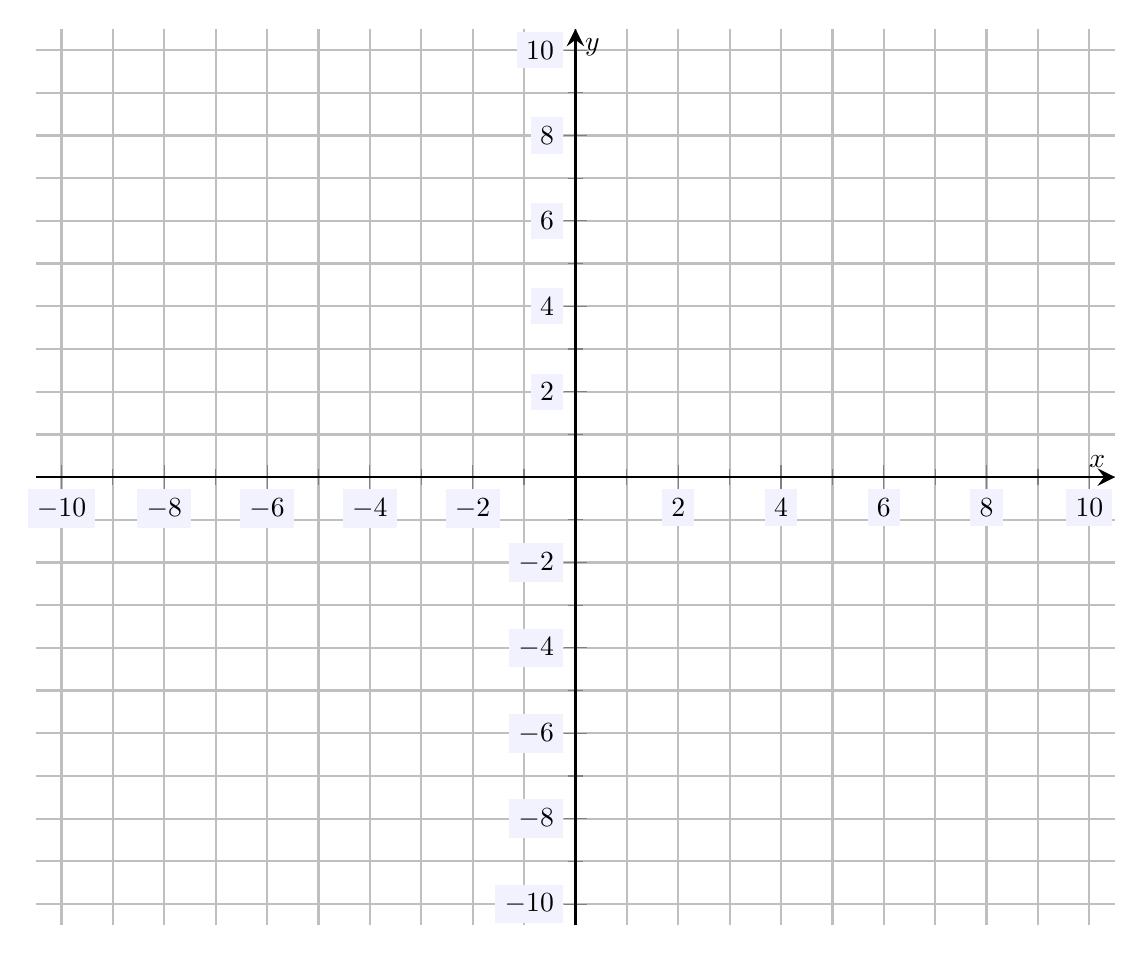
\begin{tikzpicture}[scale=2,every node/.style={scale=0.5}]
	\begin{axis}[
	grid=both,
	axis lines=middle,
	ticklabel style={fill=blue!5!white},
	xmin= -10.5, xmax=10.5,
	ymin= -10.5, ymax=10.5,
	xtick={-10,-8,-6,-4,-2,0,2,4,6,8,10},
	ytick={-10,-8,-6,-4,-2,0,2,4,6,8,10},
	minor tick = {-10,-9,...,10},
	xlabel=\(x\),ylabel=\(y\),
	]
	\end{axis}
	\end{tikzpicture}
	}
	\]



\newpage



% Problem 2
\problem{10} Sketch the function $f(x)= 8 - 2(x - 6)^2$. 
	\[
	\fbox{
	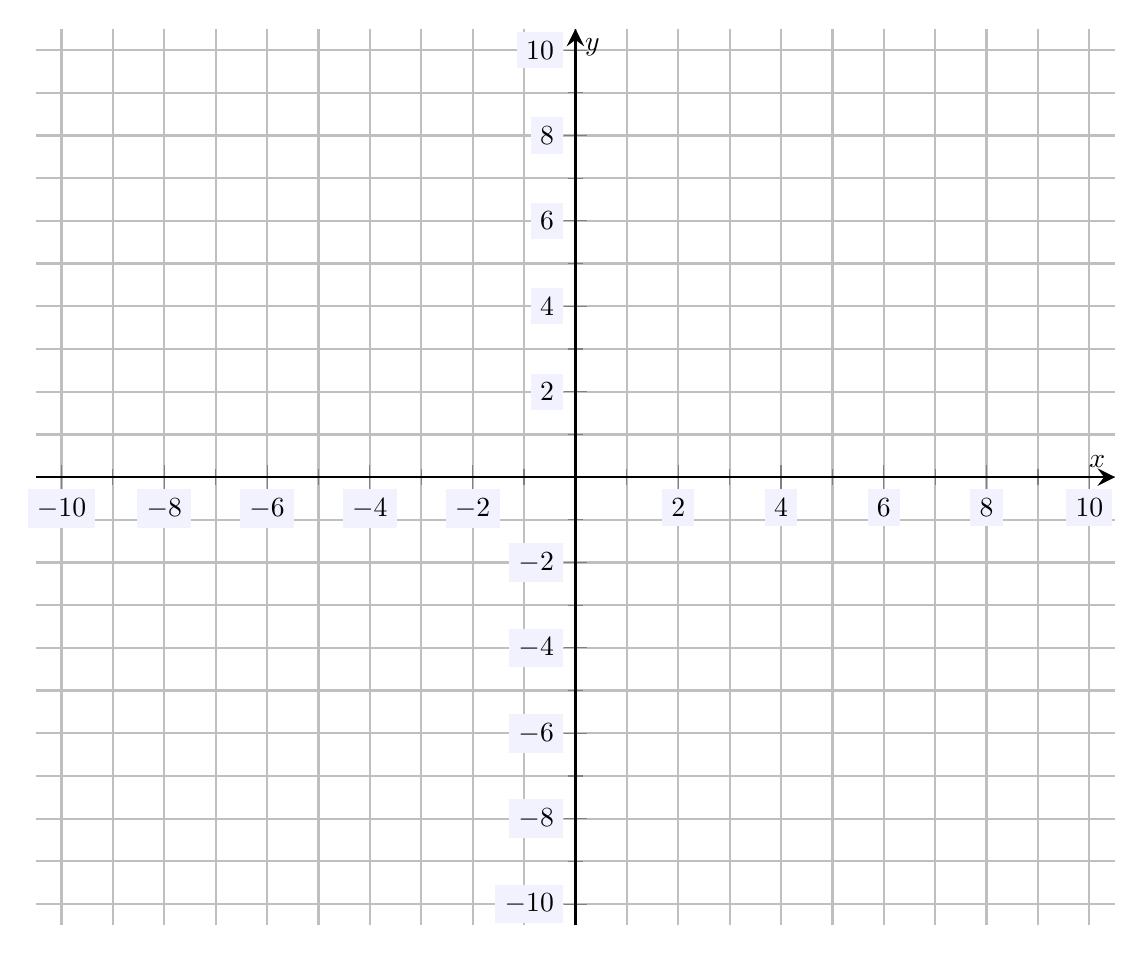
\begin{tikzpicture}[scale=2,every node/.style={scale=0.5}]
	\begin{axis}[
	grid=both,
	axis lines=middle,
	ticklabel style={fill=blue!5!white},
	xmin= -10.5, xmax=10.5,
	ymin= -10.5, ymax=10.5,
	xtick={-10,-8,-6,-4,-2,0,2,4,6,8,10},
	ytick={-10,-8,-6,-4,-2,0,2,4,6,8,10},
	minor tick = {-10,-9,...,10},
	xlabel=\(x\),ylabel=\(y\),
	]
	\end{axis}
	\end{tikzpicture}
	}
	\]



\newpage



% Problem 3
\problem{10} Sketch the function $f(x)= x^2 - 10x + 16$.
	\[
	\fbox{
	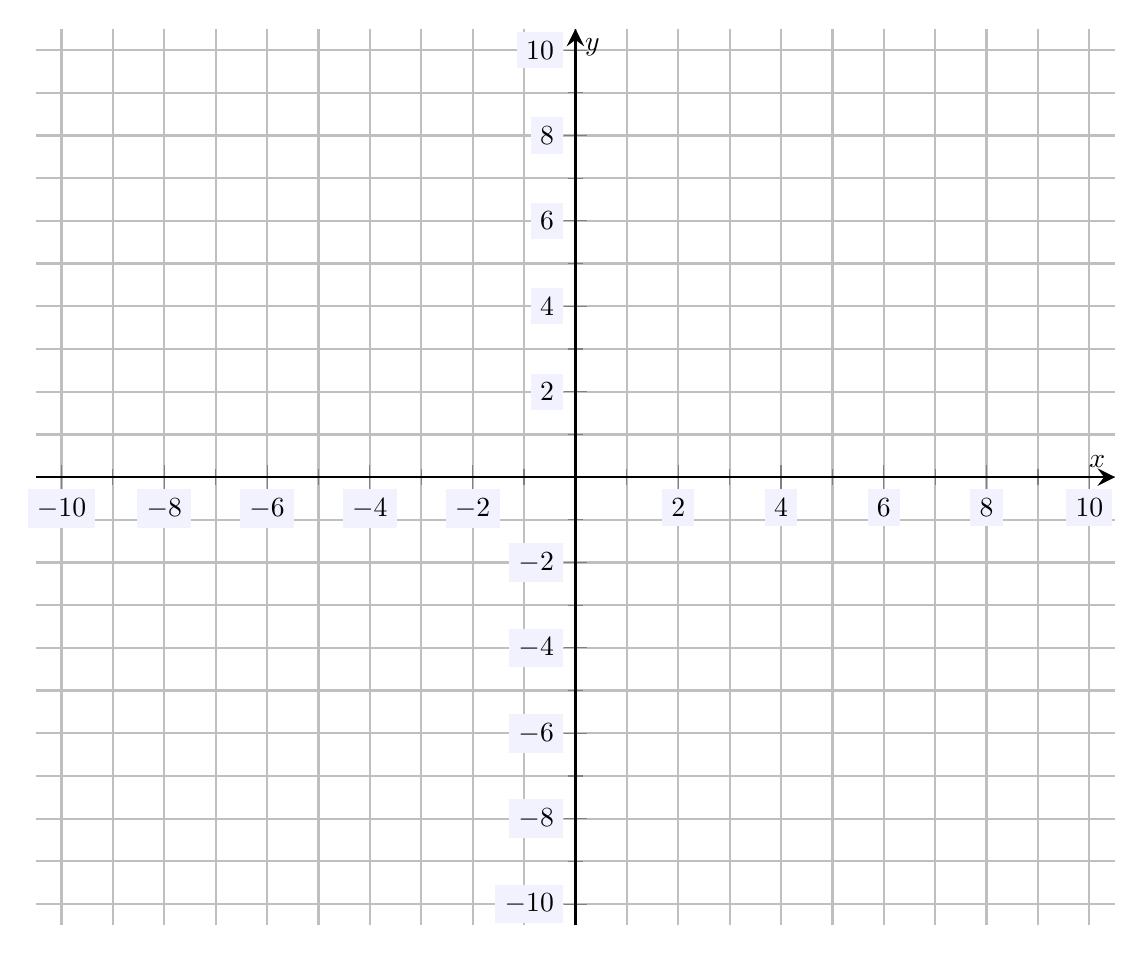
\begin{tikzpicture}[scale=2,every node/.style={scale=0.5}]
	\begin{axis}[
	grid=both,
	axis lines=middle,
	ticklabel style={fill=blue!5!white},
	xmin= -10.5, xmax=10.5,
	ymin= -10.5, ymax=10.5,
	xtick={-10,-8,-6,-4,-2,0,2,4,6,8,10},
	ytick={-10,-8,-6,-4,-2,0,2,4,6,8,10},
	minor tick = {-10,-9,...,10},
	xlabel=\(x\),ylabel=\(y\),
	]
	\end{axis}
	\end{tikzpicture}
	}
	\] 



\newpage



% Problem 4
\problem{10} Find the vertex form of $y= -2x^2 + 12x - 13$ by completing the square. \pspace



\newpage



% Problem 5
\problem{10} Find the vertex form of $y= x^2 - 12x + 48$ by the `evaluation method.' \pspace 



\newpage



% Problem 6
\problem{10} Showing all your work, factor $x^2 + 14x - 51$. \pspace



\newpage



% Problem 7
\problem{10} Showing all your work, factor $x^2 + 10x - 56$. \pspace



\newpage



% Problem 8
\problem{10} Showing all your work, factor $3x^2 + 7x - 20$. \pspace



\newpage



% Problem 9
\problem{10} Consider the quadratic function $f(x)= x^2 + 14x + 39$.
        \begin{enumerate}[(a)]
        \item Determine if the parabola opens upwards or downwards.
        \item Is the parabola convex or concave?
        \item Does the parabola have a maximum or minimum? 
        \item Find the vertex and axis of symmetry. 
        \item Find the maximum/minimum value of $f(x)$. 
        \end{enumerate} \pspace



\newpage



% Problem 10
\problem{10} Consider the quadratic function $f(x)= -2x^2 + 4x + 3$.
        \begin{enumerate}[(a)]
        \item Determine if the parabola opens upwards or downwards.
        \item Is the parabola convex or concave?
        \item Does the parabola have a maximum or minimum? 
        \item Find the vertex and axis of symmetry. 
        \item Find the maximum/minimum value of $f(x)$. 
        \end{enumerate} \pspace


\end{document}